%! TEX root = main.tex

\graphicspath{{00_Images/09_chapter/}}

\chapter{Loudspeaker Systems and Enclosures}
\label{ch:enclosures}

The bare electrodynamic driver analyzed in the preceding chapters radiates from both its front and rear faces simultaneously.
At low frequencies, where the acoustic wavelength is much larger than the diaphragm diameter, the two radiating surfaces are close enough that their contributions interfere destructively in the far field, severely limiting bass output.
The enclosure solves this fundamental problem by controlling the acoustic environment seen by the rear face of the diaphragm, allowing the front radiation to proceed unimpeded.
This chapter examines three enclosure topologies in order of increasing acoustic complexity: the unbaffled driver, the closed box, and the vented (bass-reflex) box.

\section{Unbaffled and Baffled Loudspeakers}
\label{sc:91}

\subsection{The Unbaffled Driver as a Dipole Source}
\label{ssc:911}

When a loudspeaker operates without any baffle, the diaphragm faces air on both sides.
The front face produces a positive pressure increment when it moves forward, while the rear face simultaneously produces a negative pressure increment of equal magnitude in the backward direction.
In the far field, these two contributions from a source of finite extent but vanishing dipole separation (relative to the wavelength at low frequencies) interfere destructively: air displaced forward is immediately replenished by air drawn around the driver from behind, so no net volume velocity is injected into the medium.
This effect is known as acoustic short-circuiting, and it makes the unbaffled driver behave as a dipole source rather than a monopole.
The far-field pressure of a dipole source depends on frequency, distance, and direction of observation as:
\[
p \propto \frac{f^2 U_0}{r} \cos\theta
\]
where \(U_0 = \pi a^2 u_c\) is the volume velocity, \(r\) is the observation distance, and \(\theta\) is the angle measured from the diaphragm axis.
The \(\cos\theta\) factor produces a figure-eight polar pattern: maximum sensitivity on axis (\(\theta = 0\)), zero sensitivity in the plane of the diaphragm (\(\theta = \pm 90°\)).

\paragraph{Frequency response below \(f_s\): stiffness-controlled} Below the mechanical resonance frequency, the suspension compliance dominates the impedance and the diaphragm velocity is \(u_c \propto f\), so \(U_0 \propto f\).
Substituting into the dipole pressure formula:
\[
p \propto f^2 \cdot f = f^3
\]
The pressure rises at \(+18 \mathrm{dB/oct}\) as frequency increases, or equivalently falls at \(18 \mathrm{dB/oct}\) below the stiffness-controlled cutoff.
This extremely steep rolloff makes the unbaffled driver impractical for bass reproduction.

\paragraph{Frequency response above \(f_s\): mass-controlled} Above resonance, the diaphragm mass dominates and \(u_c \propto 1/f\), so \(U_0 \propto 1/f\).
The far-field pressure then scales as:
\[
p \propto f^2 \cdot \frac{1}{f} = f
\]
Even in the mass-controlled region, the pressure still rises at \(+6 \mathrm{dB/oct}\) with increasing frequency: there is no flat passband.
This means an unbaffled driver can never achieve a constant SPL response without equalization, and the limited practical interest of the unbaffled configuration is mainly restricted to open-baffle designs used for specific aesthetic or spatial reasons.

\subsection{Baffle Configurations}
\label{ssc:912}

The fundamental purpose of any baffle or enclosure is to prevent the rear acoustic wave from canceling the front radiation.
Three idealized configurations are commonly distinguished.

\begin{figure}[!htb]
    \centering
    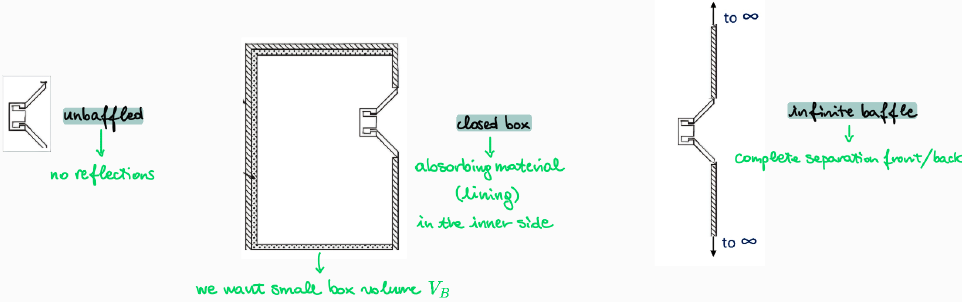
\includegraphics[width=0.80\textwidth]{baffle_configurations.png}
    \caption{Comparison of baffle configurations: unbaffled driver (left), closed-box baffle (center), and infinite baffle (right). The closed box approximates the infinite baffle in practice by enclosing the rear radiation in a sealed cabinet}
\end{figure}

The infinite baffle is the idealized case of a rigid wall of infinite extent in which the driver is mounted flush: front and rear radiation are completely separated.
The infinite baffle presents the piston radiation impedance derived in chapter \ref{ch:sound_radiation} on the front side, and zero acoustic loading on the rear.
It is not physically realizable but serves as the reference against which all practical designs are assessed.
The closed-box (sealed) baffle approximates the infinite baffle by enclosing the rear of the driver in a rigid cabinet.
The enclosed air volume introduces an additional acoustic compliance that stiffens the suspension and raises the resonance frequency, as analyzed in section \ref{sc:92}.
The vented (bass-reflex) box replaces the sealed rear panel with a tuned acoustic port, adding a second resonator that extends the usable bass response at the cost of a steeper rolloff below the system cutoff, as analyzed in section \ref{sc:93}.

\begin{figure}[!htb]
    \centering
    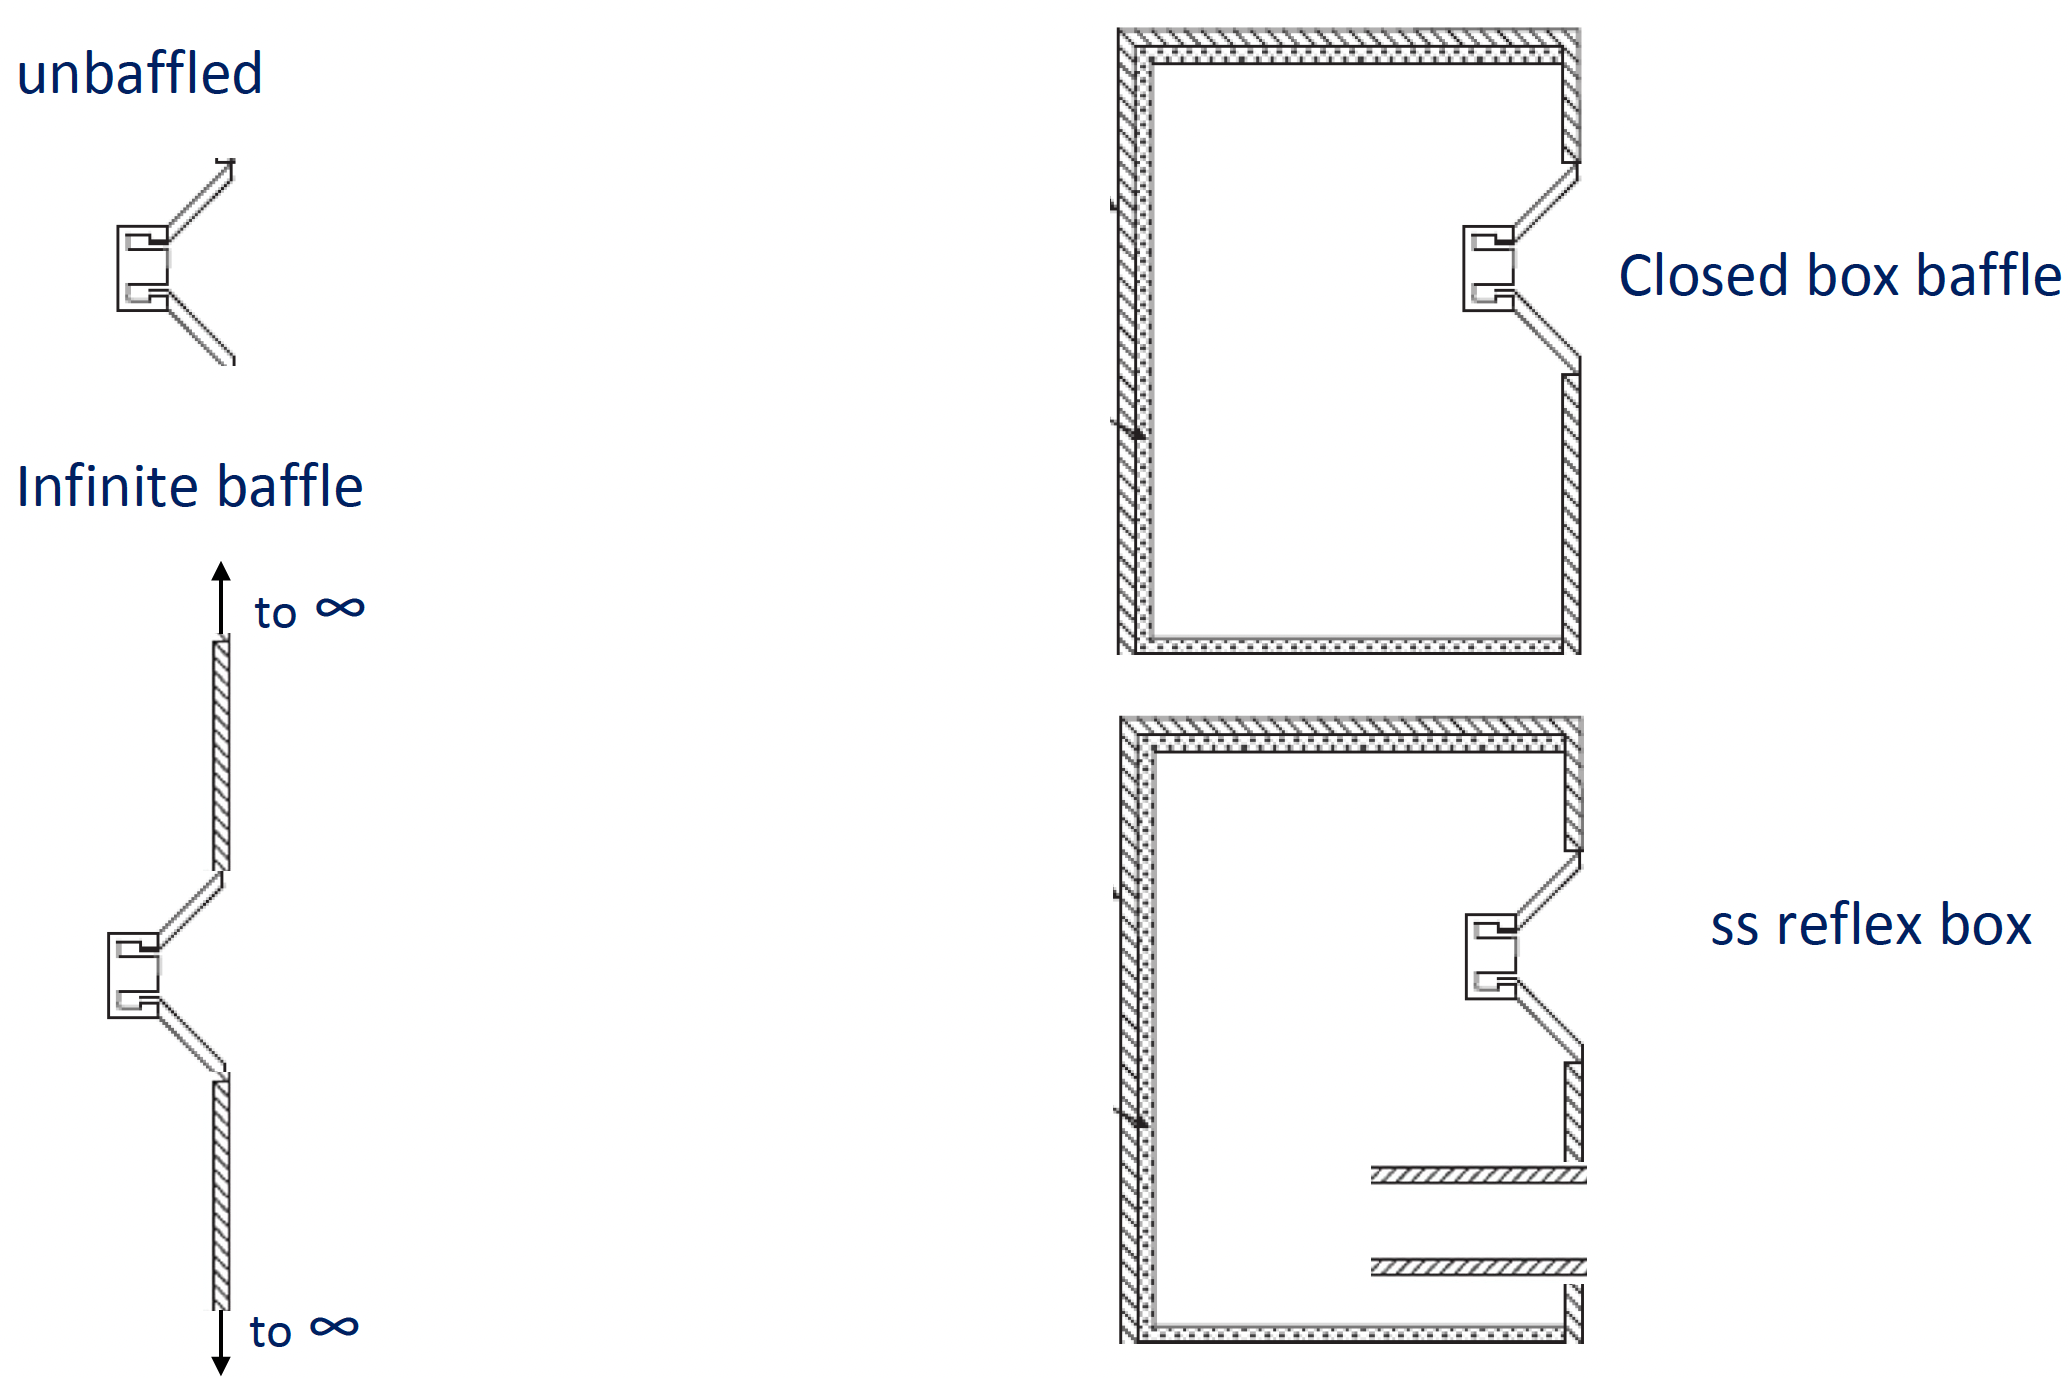
\includegraphics[width=0.70\textwidth]{baffle_types.png}
    \caption{Representative physical realizations of the three baffle topologies: open-baffle panel (left), sealed cabinet (center), and vented cabinet with front-mounted port (right)}
\end{figure}

\section{The Closed-Box Enclosure}
\label{sc:92}

The closed-box (sealed-cabinet) enclosure is the simplest practical enclosure topology.
The cabinet is made acoustically rigid, and the rear of the driver sees a sealed air volume \(V_B\).
The enclosed air behaves as an acoustic compliance:
\[
C_{AB} = \frac{V_B}{\rho_0 c^2}
\]
this is an additional mechanical compliance \(C_{MB} = C_{AB}/S_D^2\) acting in parallel with the free-air suspension compliance \(C_{MS}\).
The two compliances combine as springs in series (since stiffnesses add when compliances are in parallel electrical circuit, but the physics here means the restoring forces add, so the total compliance is reduced):
\[
C_{MSB} = \frac{C_{MS} C_{MB}}{C_{MS} + C_{MB}}
\]
Since \(C_{MSB} < C_{MS}\), the enclosed air makes the total suspension stiffer and raises the mechanical resonance frequency.

\begin{figure}[!htb]
    \centering
    \subfloat[Acoustic circuit for the box]{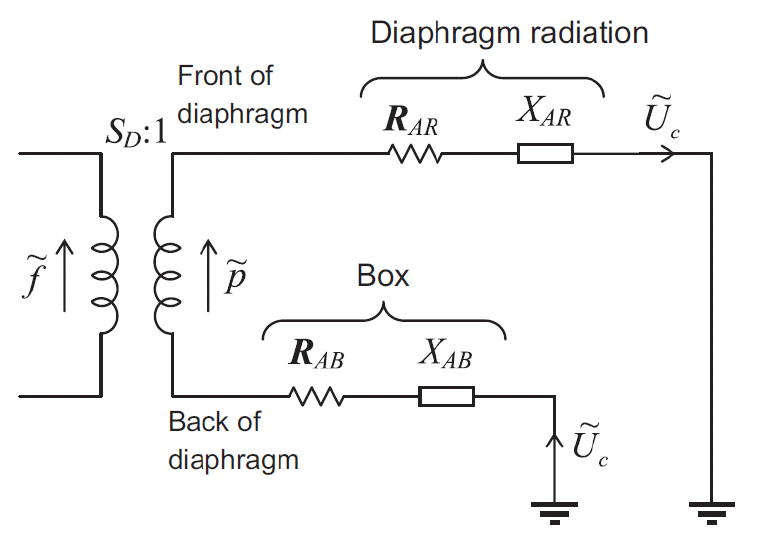
\includegraphics[height=0.16\textheight]{closed_box_circuit_1.png}}
    \hfill
    \subfloat[Complete equivalent circuit]{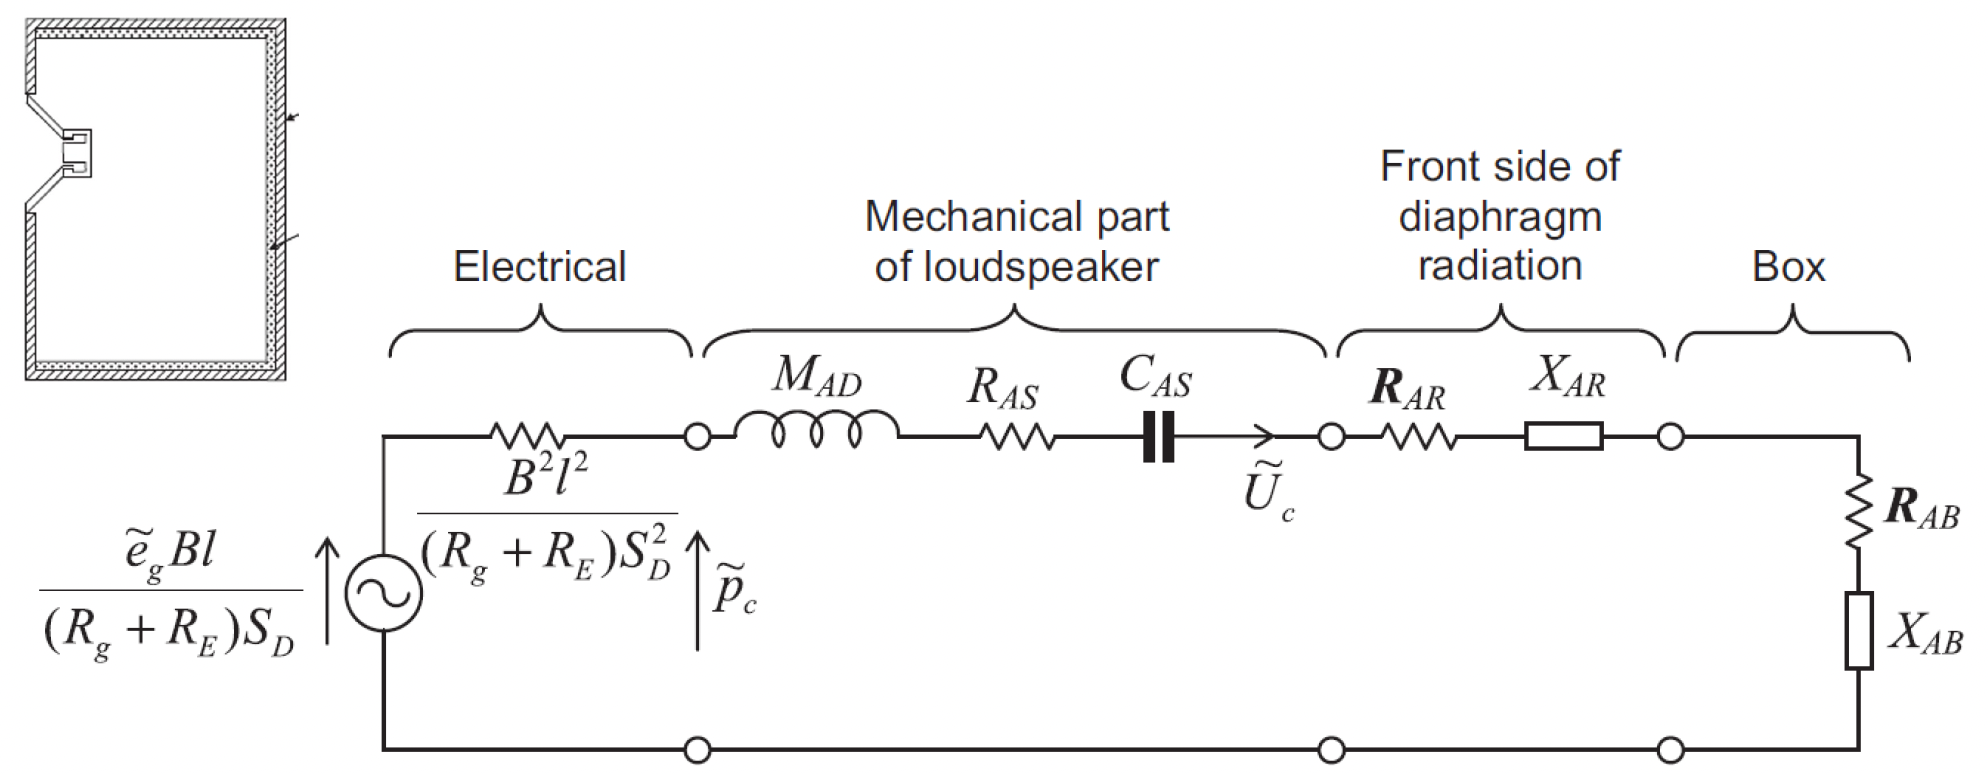
\includegraphics[height=0.16\textheight]{closed_box_circuit.png}}
    \caption{Equivalent circuits for the loudspeaker in a closed-box enclosure. The compliance \(C_{AB}\) of the air in the box appears in parallel with the mechanical suspension compliance \(C_{MS}\), stiffening the total restoring spring}
\end{figure}

\subsection{Closed-Box Resonance Frequency}
\label{ssc:921}

The closed-box resonance frequency \(f_c\) is:
\begin{equation}
    f_c = \frac{1}{2\pi\sqrt{M_{MS} C_{MSB}}}
    \label{eq:fcClosedBox}
\end{equation}
Since the equivalent compliance volume of the suspension is \(V_{AS} = C_{MS} S_D^2 \rho_0 c^2\), and the box compliance volume is \(V_B\), the combined compliance volume is:
\[
\frac{1}{V_{ASB}} = \frac{1}{V_{AS}} + \frac{1}{V_B}
\qquad\Longrightarrow\qquad
V_{ASB} = \frac{V_{AS} V_B}{V_{AS}+V_B}
\]
The ratio of closed-box to free-air resonance frequency is therefore:
\begin{equation}
    \frac{f_c}{f_s} = \sqrt{\frac{C_{MS}}{C_{MSB}}} = \sqrt{1 + \frac{V_{AS}}{V_B}}
    \label{eq:fcRatio}
\end{equation}
Equation \eqref{eq:fcRatio} is the central design relation for closed-box systems.
A box volume equal to \(V_{AS}\) raises the resonance frequency by a factor of \(\sqrt{2}\), approximately half an octave.
A smaller box produces a higher resonance and therefore a reduced bass extension, which is the fundamental trade-off in closed-box design: compactness comes at the cost of low-frequency reach.
In the limiting case of an infinitely large box (\(V_B \to \infty\)), the enclosed air has no effect and \(f_c = f_s\).
In the opposite limit of a very small box (\(V_B \ll V_{AS}\)), the box compliance dominates and the driver resonance is controlled entirely by the air spring: this is the air-suspension (acoustic-suspension) configuration, which trades bass extension for the ability to use a very compliant suspension without risk of overexcursion.

\subsection{Frequency Response and Rolloff}
\label{ssc:922}

The pressure transfer function of a loudspeaker in a closed box is a second-order high-pass filter with the closed-box resonance \(f_c\) and total quality factor \(Q_{TC}\):
\[
\tilde{p}(r) = -\frac{\tilde{e}_g Bl S_D}{(R_g + R_E) M_{MS}} \frac{e^{-jkr}}{4\pi r} \alpha_C(f),
\qquad
\alpha_C(f) = \frac{-(f/f_c)^2}{1 - (f/f_c)^2 + j (f/f_c)/Q_{TC}}
\]
The normalized transfer function \(|\alpha_C(f)|\) is flat well above \(f_c\), peaks at \(f_c\) with a height determined by \(Q_{TC}\), and falls at \(-12 \mathrm{dB/oct}\) below \(f_c\).
This second-order rolloff slope is an intrinsic property of the closed-box topology and cannot be changed without modifying the order of the system.
The total quality factor is:
\[
Q_{TC} = \frac{Q_{EC} Q_{MC}}{Q_{EC} + Q_{MC}}, \qquad Q_{MC} = Q_{MS}\sqrt{1 + \frac{V_{AS}}{V_B}}
\]
The critically damped response (\(Q_{TC} = 1/\sqrt{2} \approx 0.707\)) provides the maximally flat (Butterworth) alignment and is the standard design target for most home-audio closed-box systems.
Values of \(Q_{TC}\) above unity produce a peaked response at \(f_c\) that sounds "boomy" while narrowing the effective bandwidth; values below 0.5 are overdamped and roll off early, giving a thinner bass character.

\begin{figure}[!htb]
    \centering
    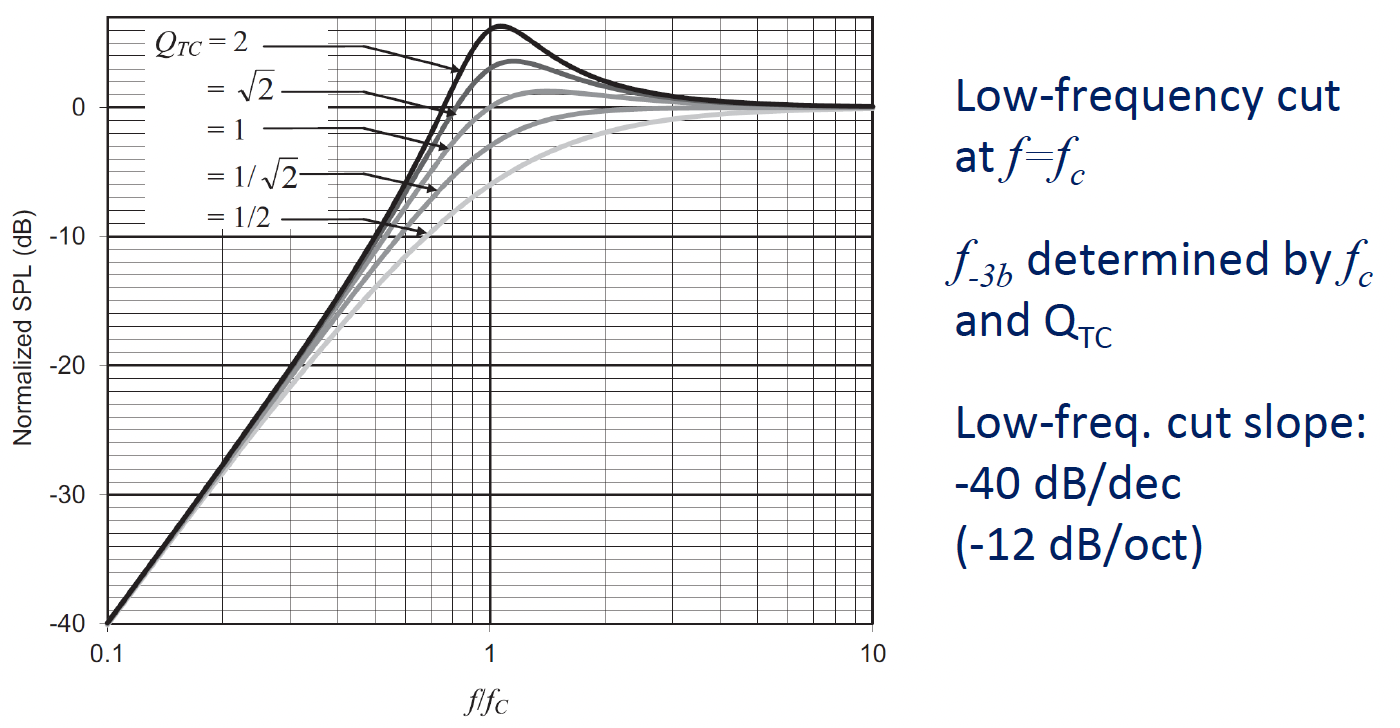
\includegraphics[width=0.55\linewidth]{closed_box_SPL.png}
    \caption{Normalized SPL frequency response of a loudspeaker in a closed-box enclosure for several values of \(Q_{TC}\). The second-order high-pass rolloff of \(-12 \mathrm{dB/oct}\) below \(f_c\) is independent of \(Q_{TC}\); the quality factor determines only the shape of the transition region around \(f_c\)}
\end{figure}

\section{The Bass-Reflex (Vented) Enclosure}
\label{sc:93}

The bass-reflex, or vented-box, enclosure adds an acoustic port to the cabinet: a duct (tube) or slot that connects the interior air volume to the exterior.
The port introduces an additional resonator that can reinforce the bass output below the driver's free-air resonance, extending the usable low-frequency bandwidth compared to a closed-box system of the same volume.
The price paid for this extension is a steeper rolloff below the system cutoff, as will be seen below.

\begin{figure}[!htb]
    \centering
    \subfloat[Schematic model]{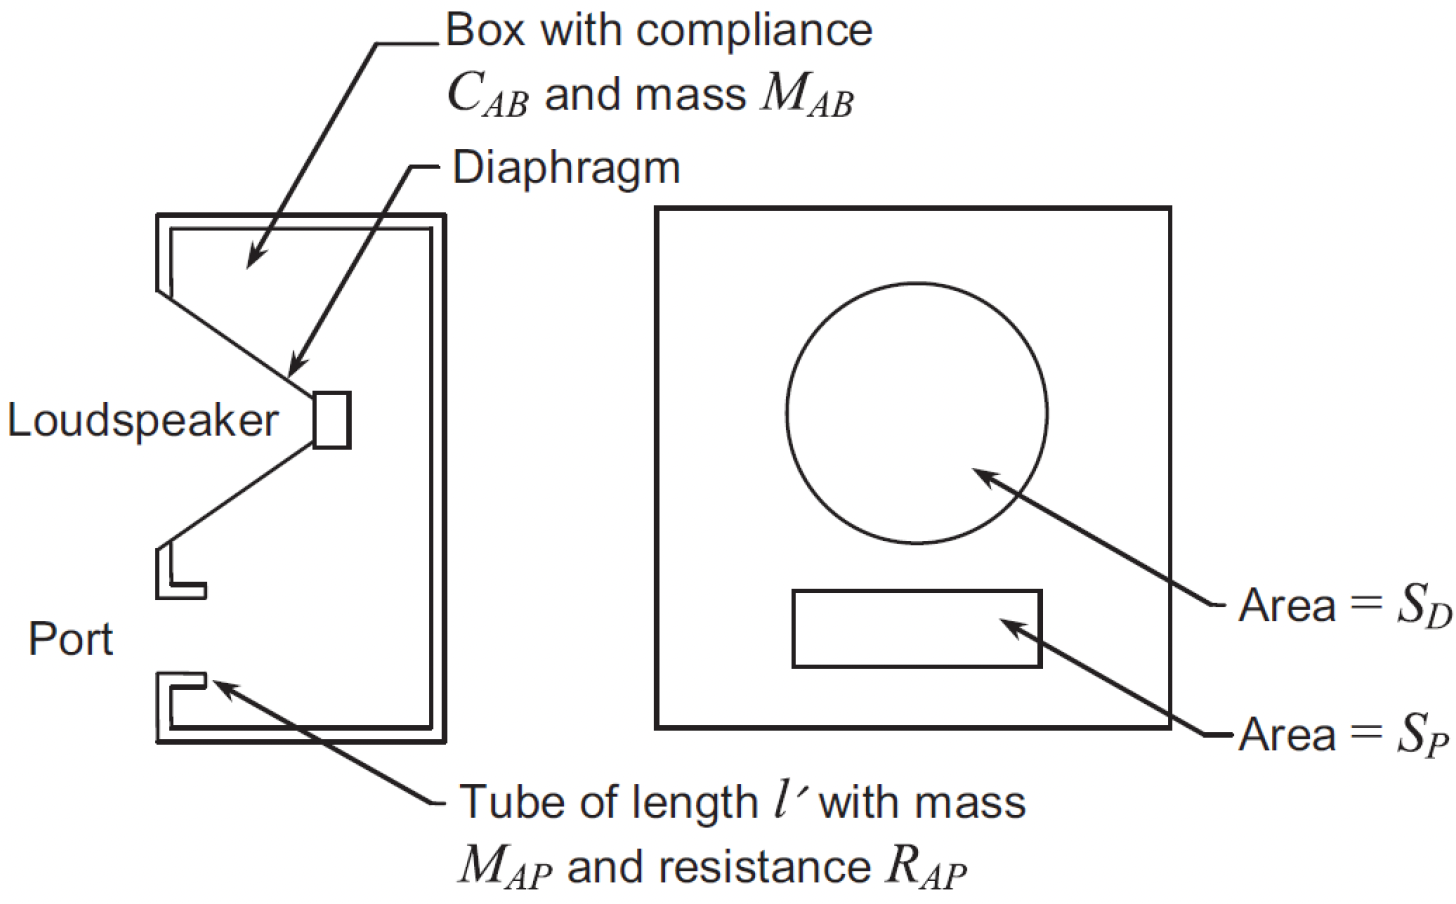
\includegraphics[height=0.22\textheight]{bass_reflex_model.png}}
    \hspace{1cm}
    \subfloat[Air masses and compliances]{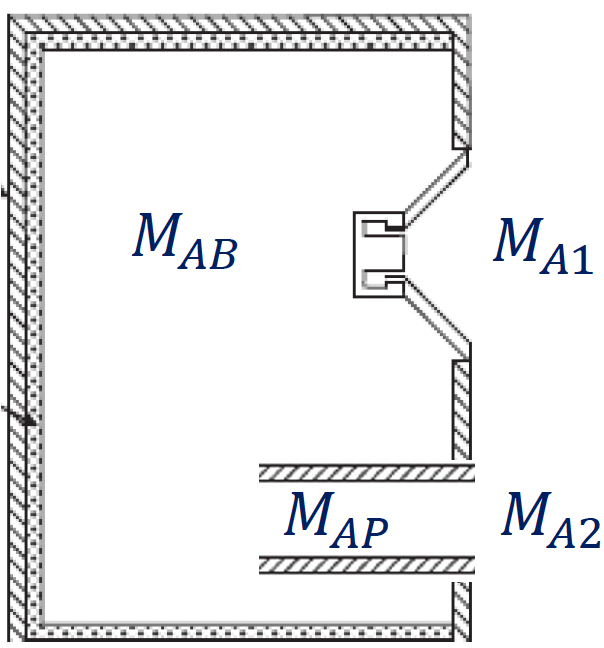
\includegraphics[height=0.22\textheight]{bass_reflex_air_masses.png}}
    \caption{The bass-reflex enclosure. The port duct of cross-section \(S_P\) and length \(t\) provides the acoustic mass \(M_{AT}\); the enclosed air volume \(V_B\) provides the acoustic compliance \(C_{AB}\). Together they form a Helmholtz resonator tuned to the port frequency \(f_B\)}
\end{figure}

\subsection{The Helmholtz Resonator Formed by the Port}
\label{ssc:931}

The air inside a circular port tube of cross-section \(S_P\) and effective length \(t\) (including end corrections) behaves as a lumped acoustic mass:
\[
M_{AT} = \frac{\rho_0 t}{S_P}
\]
The enclosed air volume \(V_B\) provides the acoustic compliance:
\[
C_{AB} = \frac{V_B}{\rho_0 c^2}
\]
Together, \(M_{AT}\) and \(C_{AB}\) form a Helmholtz resonator whose resonance frequency is:
\[
f_B = \frac{1}{2\pi\sqrt{M_{AT} C_{AB}}} = \frac{c}{2\pi}\sqrt{\frac{S_P}{V_B t}}
\]
The port frequency \(f_B\) is the key design parameter of a vented box.
In a typical design it is set close to the driver's free-air resonance \(f_s\), so that the two coupled resonances, one associated with the moving mass \(M_{MS}\) and one with the air mass \(M_{AT}\), produce a flat extended response in the transition band.

\subsection{Behavior at the Port Resonance Frequency}
\label{ssc:932}

The most physically striking property of the bass-reflex system is what happens at \(f_B\): the acoustic impedance of the box-plus-port branch rises to its maximum (the parallel LC resonator is at resonance and presents a very high impedance), so almost no volume velocity flows into the box from the diaphragm.
Instead, the large volume velocity is supplied entirely by the port, which at \(f_B\) oscillates in phase with the front radiation of the driver.
The result is that at the port resonance frequency the diaphragm motion is nearly zero (it is effectively stopped by the back-pressure from the box), while the port radiates the acoustic output.
This is both the strength and the vulnerability of the bass-reflex design: the cone is mechanically unloaded at \(f_B\), so it cannot thermally or mechanically fail, but below \(f_B\) the back-pressure disappears and the cone is free to move with very large excursion, a danger zone for the driver if the signal content extends well below \(f_B\).

\begin{figure}[!htb]
    \centering
    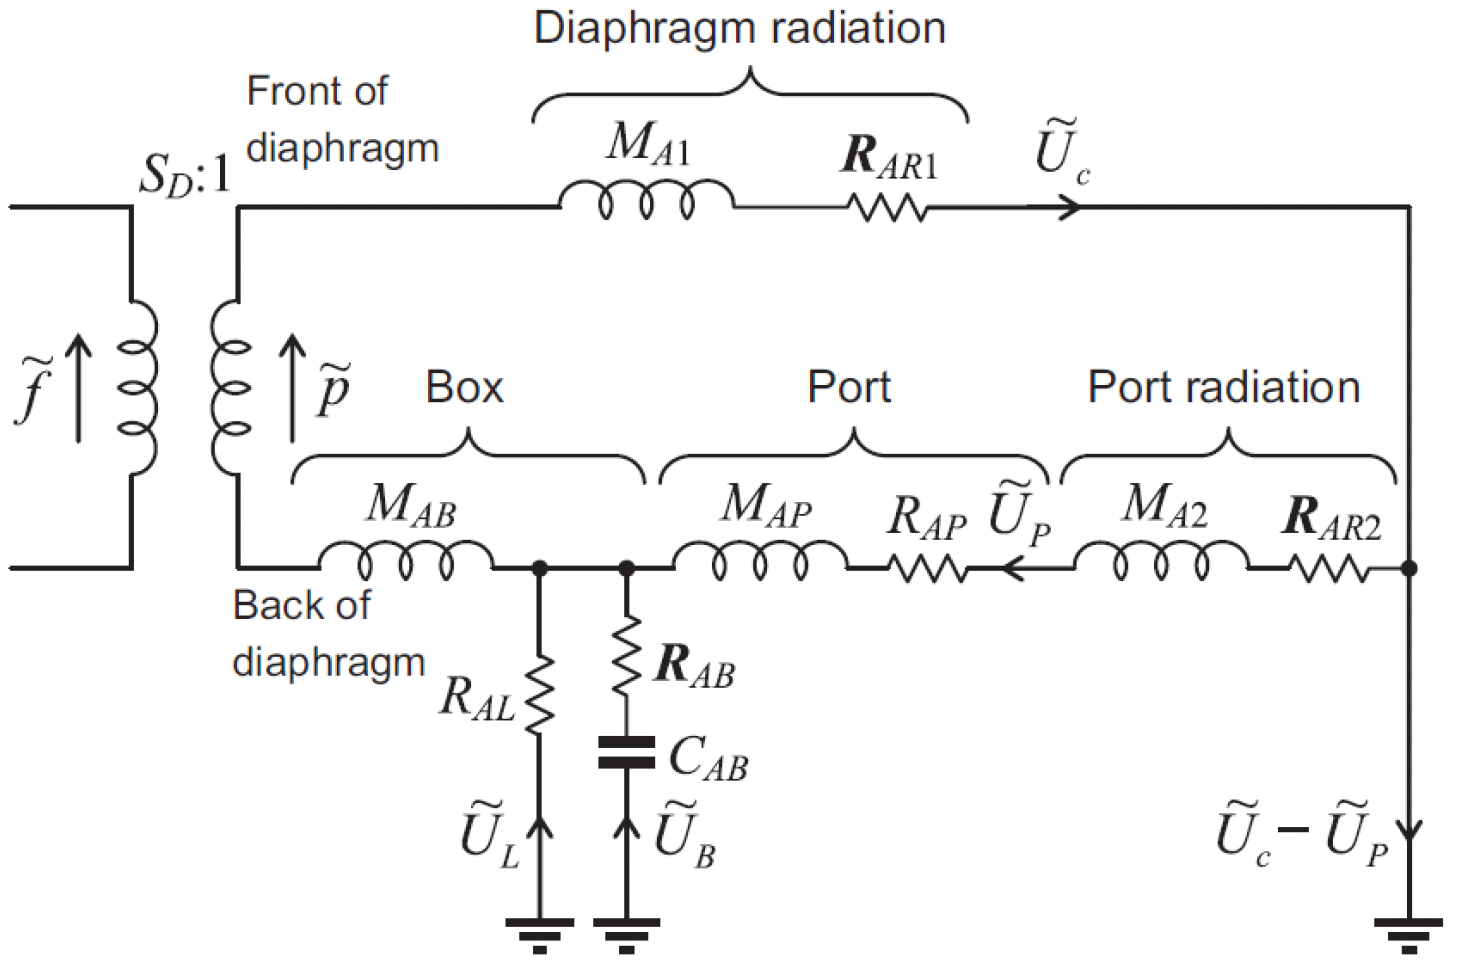
\includegraphics[width=0.70\textwidth]{bass_reflex_circuit.png}
    \caption{Equivalent electro-mechano-acoustic circuit of the bass-reflex loudspeaker. The diaphragm branch (series RLC) and the port branch (parallel LC with compliance \(C_{AB}\) and mass \(M_{AT}\)) are coupled through the box compliance. At \(f_B\) the port branch resonates and presents infinite impedance, stopping the diaphragm and maximizing port output}
\end{figure}

\subsection{Transfer Function and Rolloff Slope}
\label{ssc:933}

The pressure radiated by the combined diaphragm and port is governed by a fourth-order transfer function of the form:
\[
G(s) = \frac{s^4}{s^4 + P_3 s^3 + P_2 s^2 + P_1 s + P_0}
\]
where the coefficients \(P_0\) through \(P_3\) depend on \(\omega_s\), \(\omega_B\), \(Q_{TS}\), and the volume ratio \(V_{AS}/V_B\).
The fourth-order numerator is the defining characteristic of the vented-box topology: it produces a rolloff below the system cutoff of \(-24 \mathrm{dB/oct}\) (or \(-80 \mathrm{dB/dec}\)), steeper by one complete octave-slope than the closed box.
This steeper rolloff protects the driver from infrasonic content above the cutoff but exposes it to large excursions below it, reinforcing the importance of a high-pass filter in the signal chain.

\begin{figure}[!htb]
    \centering
    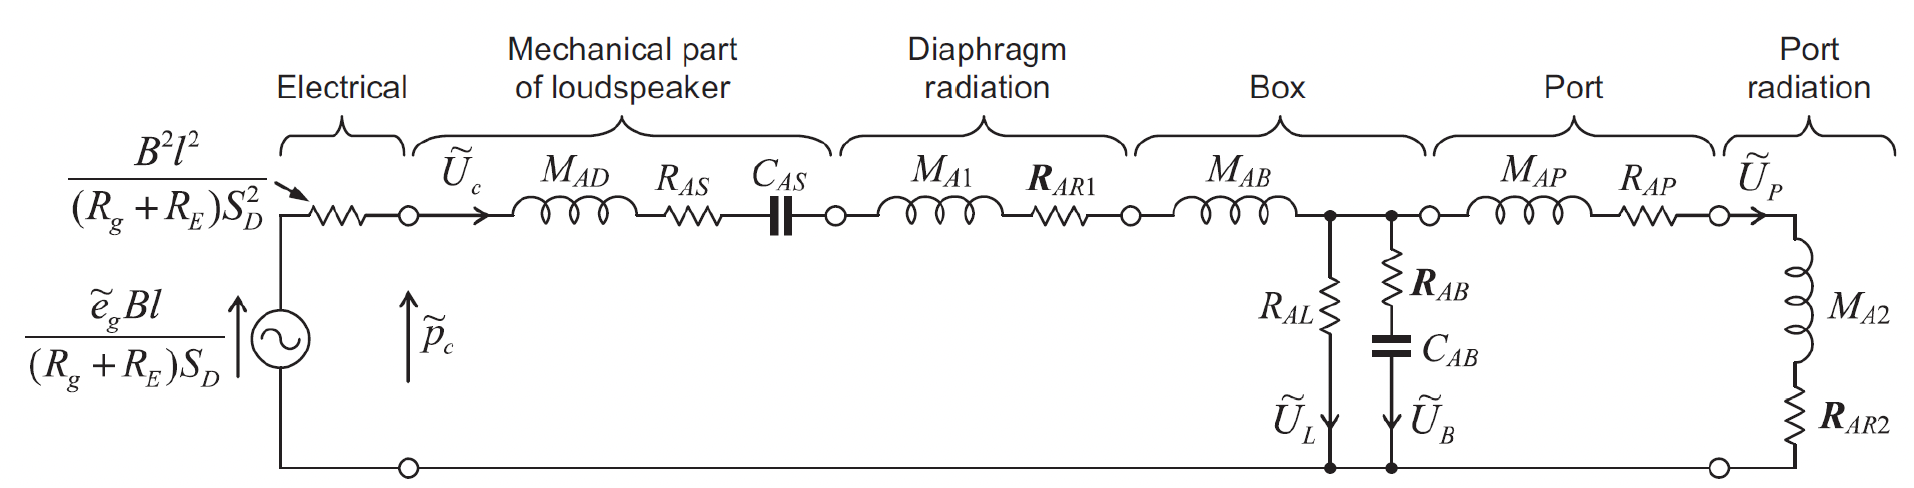
\includegraphics[width=0.90\textwidth]{bass_reflex_complete_scheme.png}
    \caption{Complete schematic representation of the bass-reflex system showing the driver, cabinet, port, and their equivalent-circuit elements. The system has two characteristic frequencies \(\omega_s\) and \(\omega_B\) and a total quality factor \(Q_{TS}\) that together determine the alignment}
\end{figure}

\subsection{Comparison: Closed Box versus Bass-Reflex}
\label{ssc:934}

The two enclosure topologies present a fundamental performance trade-off.
The bass-reflex alignment extends the usable bass response by up to a factor of 1.4 (half an octave) compared to the closed-box alignment for the same driver in the same cabinet volume, because the port resonance adds a second mode that fills in the response below the driver's natural resonance.
On the other hand, the steeper \(-24 \mathrm{dB/oct}\) rolloff below the tuning frequency means that the bass-reflex system is more sensitive to infrasonic transients (thumps, rumble), which can produce very large unloaded cone excursions that exceed the driver's mechanical limits.

\begin{figure}[!htb]
    \centering
    \subfloat[On-axis SPL responses for selected alignments]{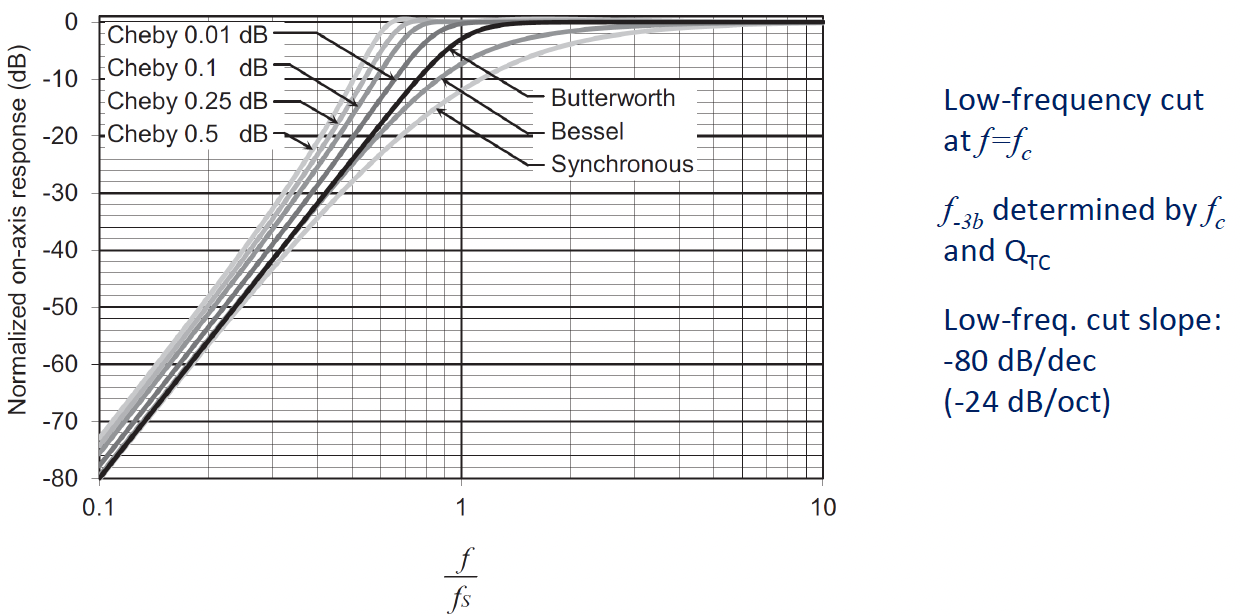
\includegraphics[width=0.46\linewidth]{bass_reflex_SPL.png}}
    \hfill
    \subfloat[Separate contributions of cone and port]{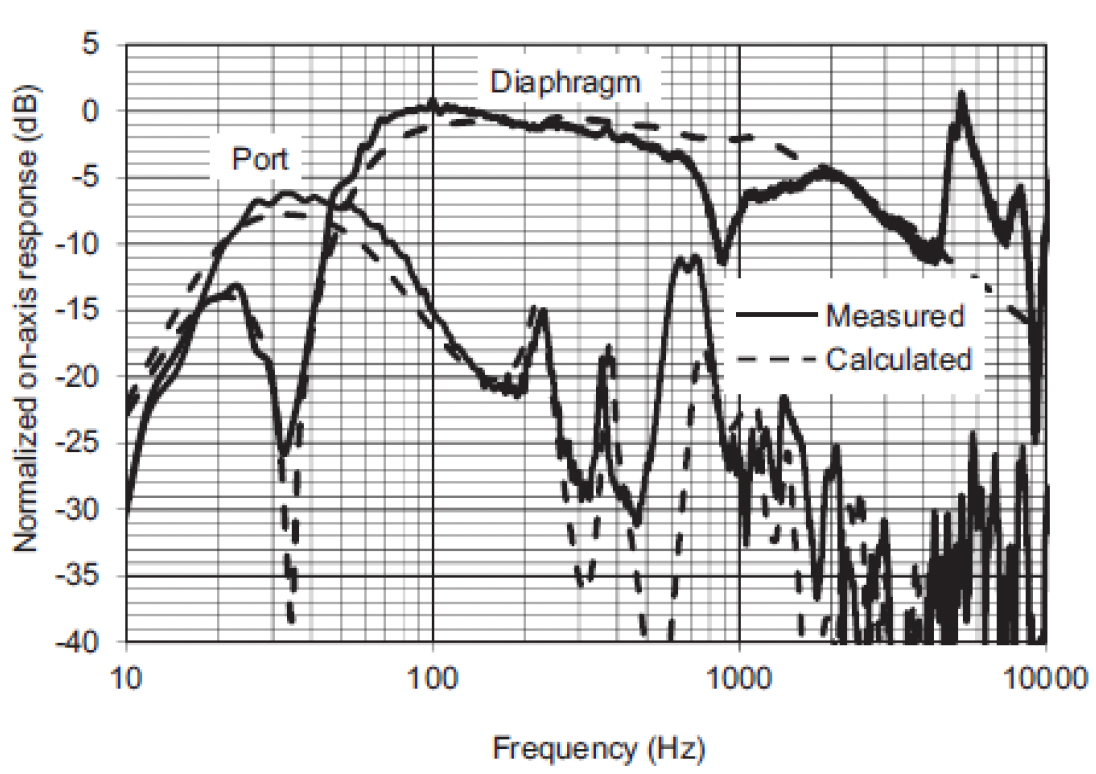
\includegraphics[width=0.46\linewidth]{bass_reflex_SPL_on_axis.png}}
    \caption{Frequency response of the bass-reflex system. The total SPL (left) shows the fourth-order high-pass rolloff of \(-24 \mathrm{dB/oct}\) below the tuning frequency. The individual contributions (right) show that the port dominates the output near \(f_B\) while the driver dominates above and below}
\end{figure}

The selection between the two topologies depends on the application.
Closed-box systems are preferred when group-delay accuracy, resistance to overexcursion, and compact dimensions are paramount.
Bass-reflex systems are preferred when maximum SPL output and extended bass in a given cabinet volume are the primary requirements, and when appropriate crossover filtering can protect the driver below tuning.
